\chapter{System Development and Implementation}

This chapter describes the system development and implementation in the same order as the project work. First, the frame-based vision system on the Jetson was established. Second, offline event-based object detection with RVT was validated on the Jetson. After that, the Kria KV260 and IMX636 event-camera platform was set up. Finally, a real-time event processing system between the Kria and Jetson was built.

\section{Frame-Based Vision System on Jetson}

The goal of the first project stage was to build a traditional vision processing pipeline that could run and be measured. This stage established methods for object tracking, offline dataset evaluation, and runtime measurement, and provided an engineering baseline for the later event-based vision system.

The frame-camera stage used an Intel RealSense D435i as the input device. Camera input, model inference, bounding-box display, and result output were completed. Several detection networks were tested with the \texttt{jetson-inference} framework~\parencite{jetsonInference,jetsonInferenceBuild}, including SSD-MobileNet-v2, SSD-Inception-v2, PeopleNet, DashCamNet, and TrafficCamNet. The program uses \texttt{videoSource} to obtain camera or image input, \texttt{detectNet} to perform TensorRT inference, and \texttt{videoOutput} to display or save the results. Figure~\ref{fig:rgb_live_ssd} shows one example of SSD-MobileNet-v2 running on real-time camera input.

\begin{figure}[htbp]
    \centering
    \IfFileExists{images/rgb_live_ssd_mobilenet_v2.png}{
        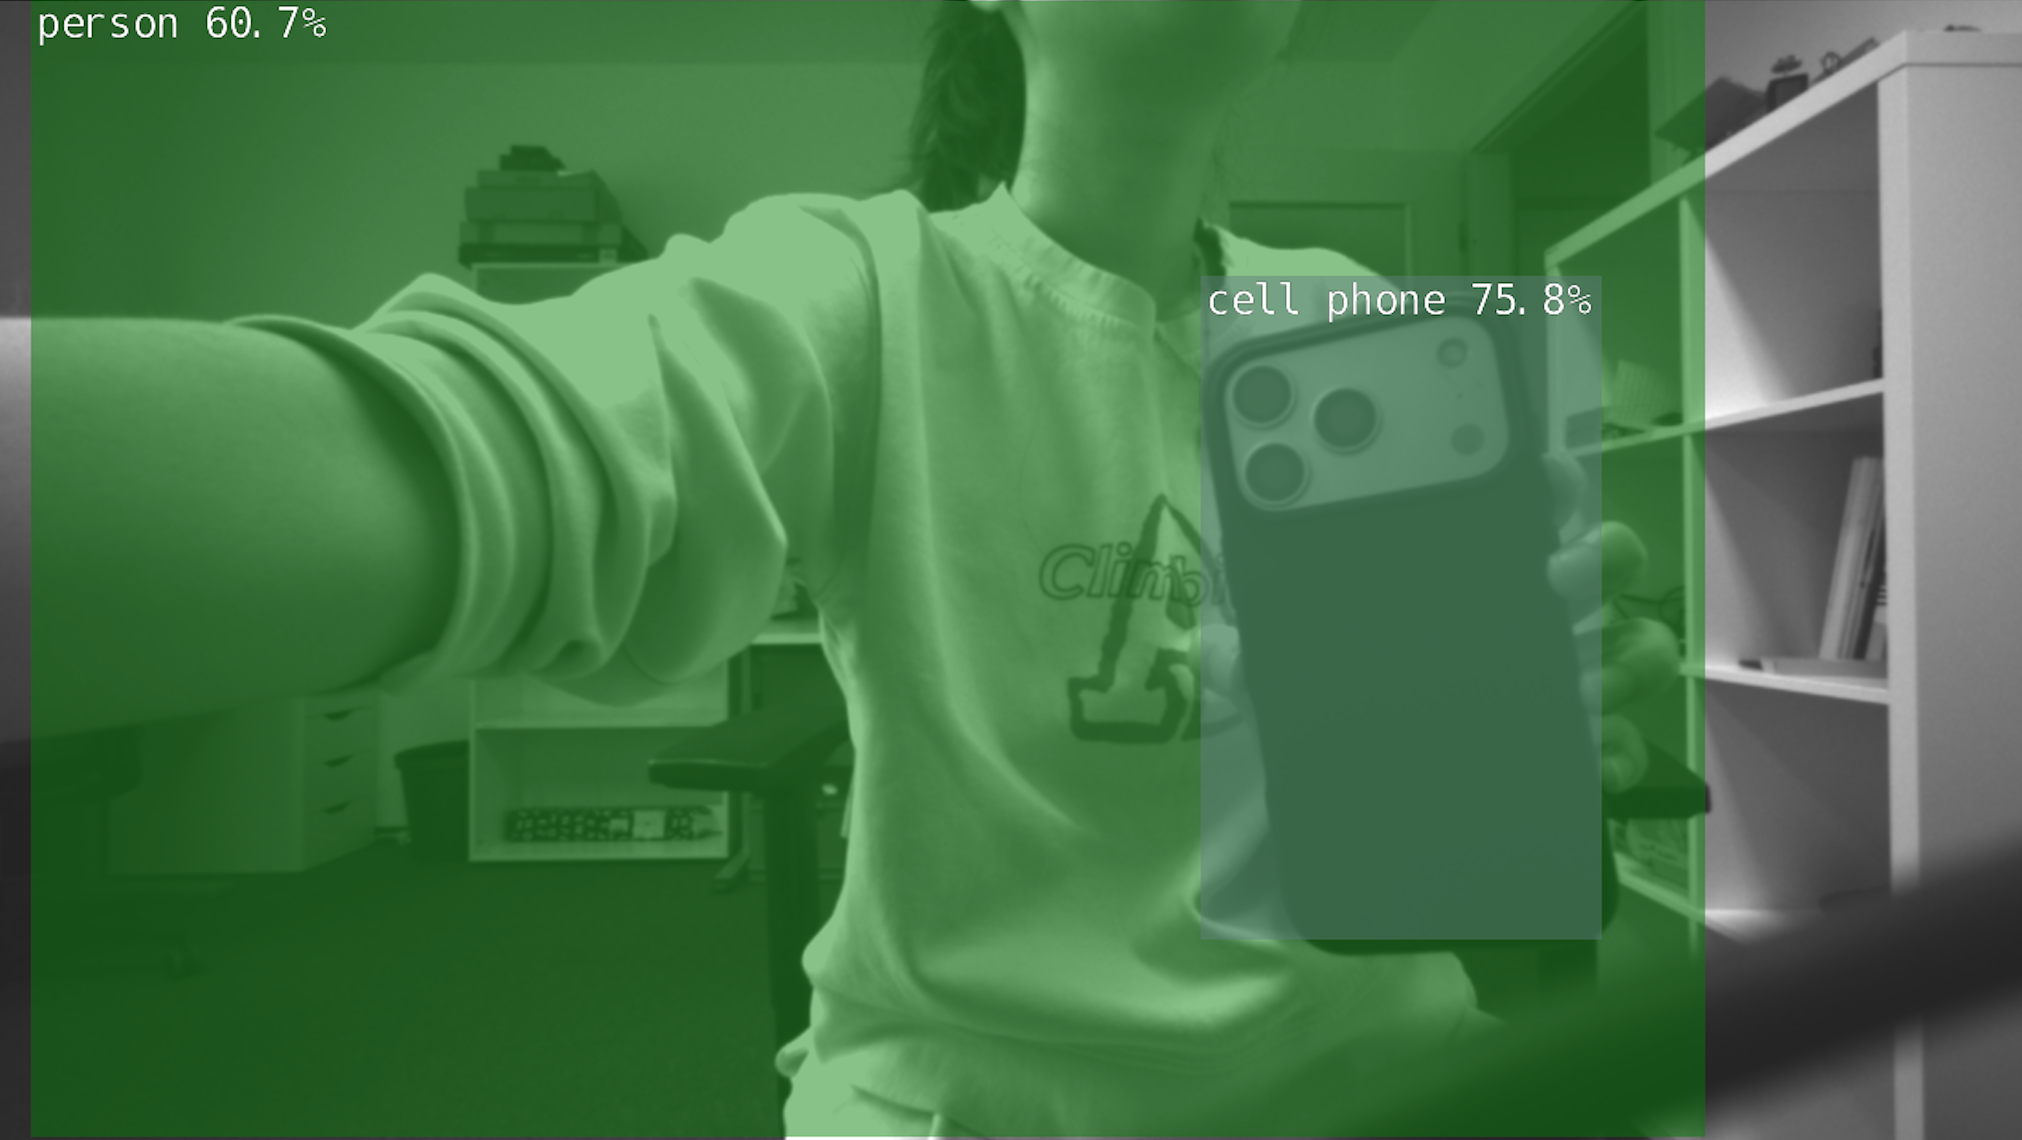
\includegraphics[width=0.88\textwidth]{images/rgb_live_ssd_mobilenet_v2.png}
    }{
        \fbox{\parbox[c][0.22\textheight][c]{0.82\textwidth}{\centering Image to be uploaded: \texttt{rgb\_live\_ssd\_mobilenet\_v2.png}}}
    }
    \caption{Detection result of SSD-MobileNet-v2 on real-time input from the RealSense D435i.}
    \label{fig:rgb_live_ssd}
\end{figure}

This figure is mainly used to show that real-time input, object detection, and result display can form a continuous processing pipeline on the Jetson. The detection boxes in the figure are qualitative examples. Runtime measurements and detection evaluation are performed with separate test procedures.

Based on the object detection system, a C++ object tracking program was built. The program mainly contains four parts: input, detection, tracking, and output. \texttt{videoSource} reads the current frame, \texttt{detectNet} produces detection boxes, \texttt{objectTrackerIOU} keeps the track ID based on the IoU relationship between detection boxes in neighboring frames, and \texttt{videoOutput} displays or saves the final result. This method has a low computational cost and is suitable as a basic tracking solution on an embedded platform. However, when objects move quickly, are occluded, or cross each other, tracking based only on IoU has limited association ability. Therefore, this project uses it as a basic tracking prototype.

To move from only displaying detection boxes to quantitative evaluation, a KITTI image batch-processing program was established. The program reads images from the KITTI object detection dataset, performs warm-up, runs DetectNet inference, saves prediction visualizations and text results, and reads the corresponding ground-truth annotations. Predicted boxes and ground-truth boxes are matched one-to-one according to IoU when their classes are the same. TP, FP, and FN are then counted, and Precision, Recall, and F1 are calculated. This process is mainly used to verify the complete workflow of detection, result saving, matching, and evaluation, and also provides a unified method for later performance tests.

Figure~\ref{fig:kitti_examples} shows two KITTI frame-based vision examples to give a direct view of the DetectNet object detection results. The bounding boxes show the object positions predicted by the model. The class names and percentages next to the boxes show the predicted classes and their confidence scores.

\begin{figure}[htbp]
    \centering
    \begin{subfigure}[t]{0.48\textwidth}
        \centering
        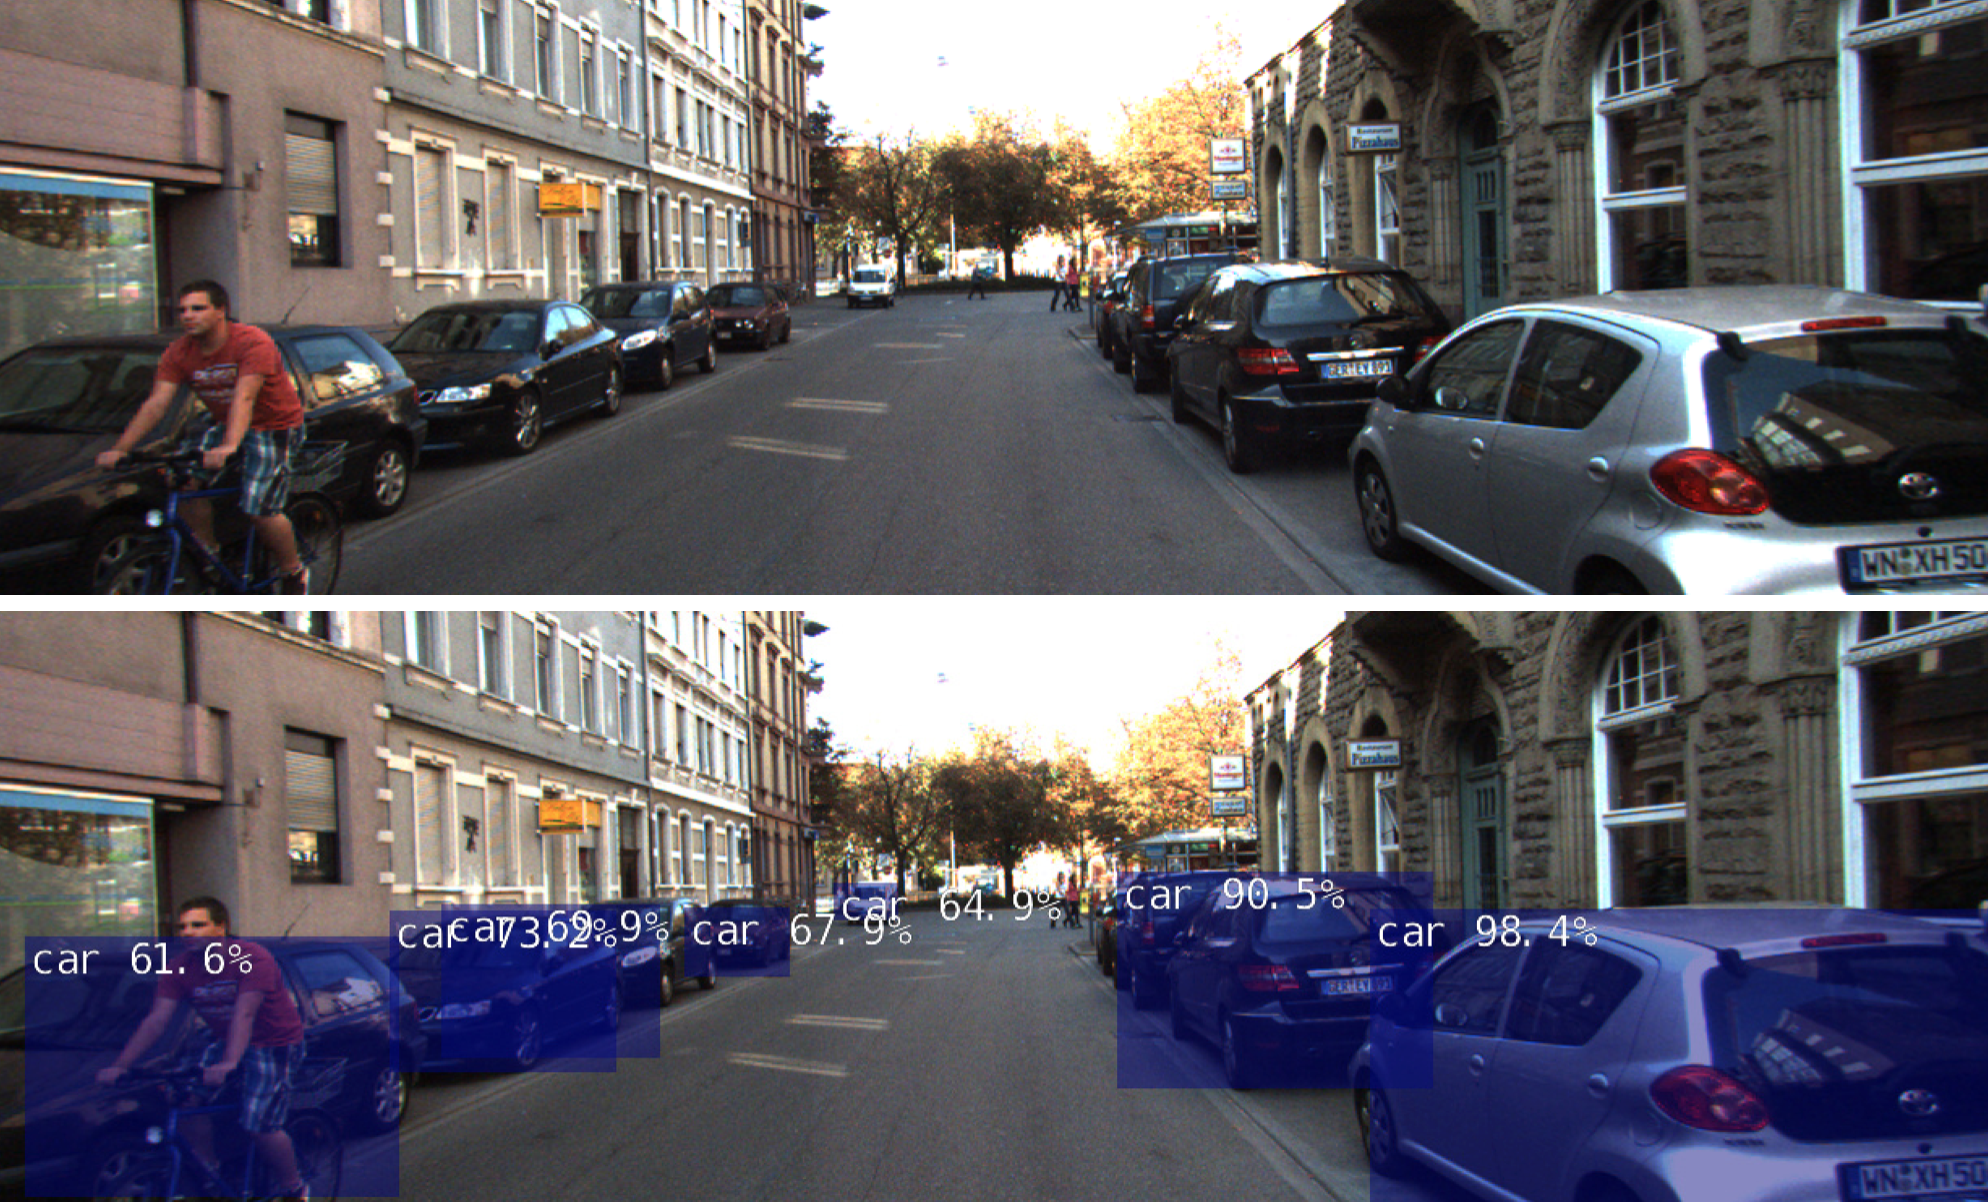
\includegraphics[width=\linewidth]{images/gen1_sample_01.png}
        \caption{KITTI example 1}
    \end{subfigure}
    \hfill
    \begin{subfigure}[t]{0.48\textwidth}
        \centering
        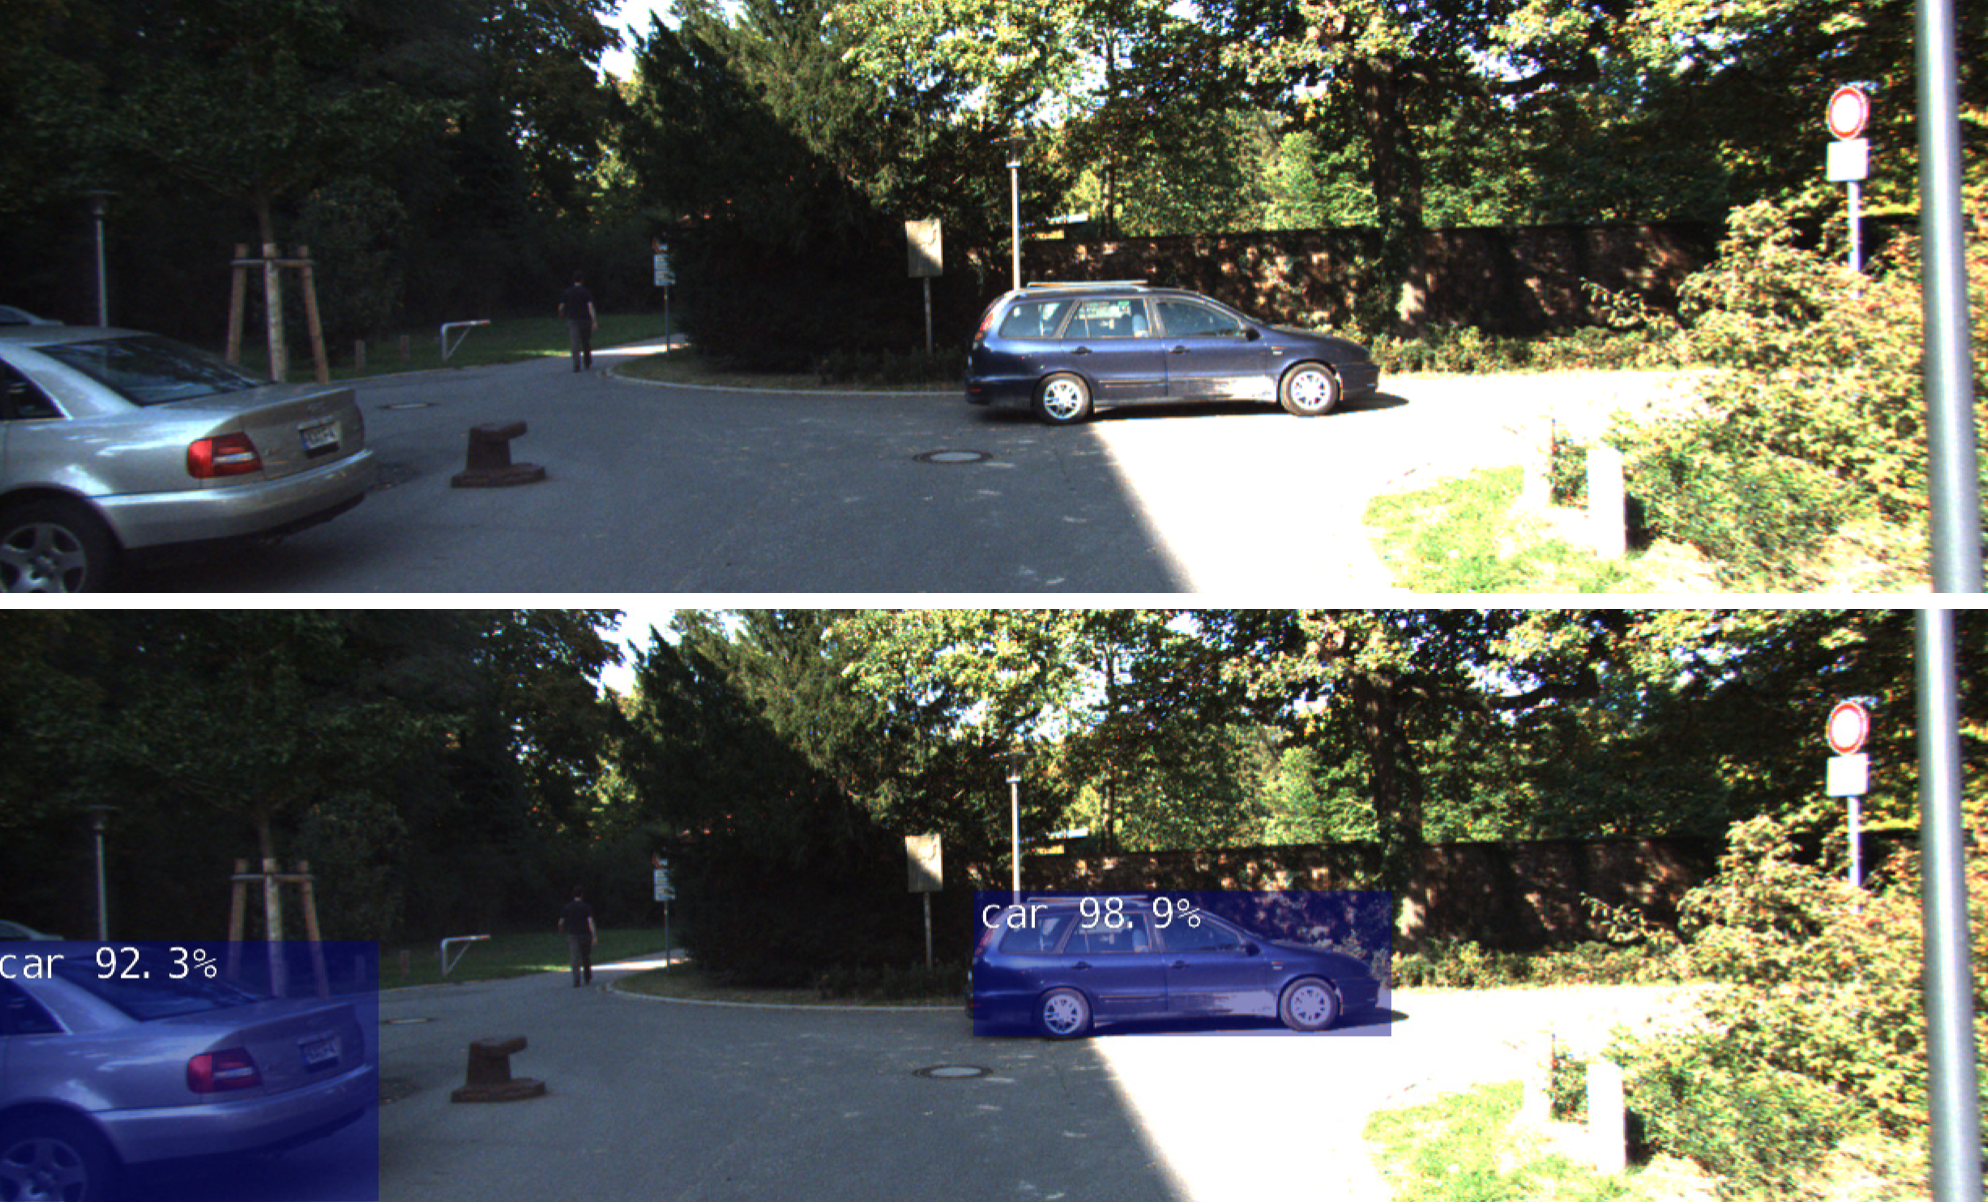
\includegraphics[width=\linewidth]{images/gen1_sample_02.png}
        \caption{KITTI example 2}
    \end{subfigure}
    \caption{Visualization examples of KITTI frame-based object detection and ground-truth annotations.}
    \label{fig:kitti_examples}
\end{figure}

\section{Offline Event-Based Object Detection with RVT on Jetson}
\label{sec:rvt_offline}

The second stage changed the research focus from frame-based vision to event-based object detection. To avoid introducing sensor, network, and model variables at the same time before the real camera pipeline was completed, this project first used offline GEN1 data to verify that RVT could run on the Jetson platform. This part is kept as an independent event-based object detection validation and is not directly connected to the final real-time event pipeline.

The official RVT implementation was originally developed for normal GPU and Conda environments, while the Jetson uses the ARM64 architecture and the JetPack software environment. Therefore, the deployment required compatible PyTorch and CUDA versions and controlled versions of the other dependencies. A reproducible RVT runtime environment was finally established. CUDA availability was confirmed, the Hydra configuration could be loaded, and the GEN1 data and checkpoint could be read correctly. This project uses preprocessed Prophesee GEN1 data and the RVT-Tiny GEN1 checkpoint provided by the official RVT repository~\parencite{rvtGithub}. The GEN1 data uses a preprocessed stacked-histogram event representation with a time window of about 50 ms and 10 time bins. During validation, \texttt{batch\_size.eval=1} is used, which means that only one sample is processed at a time to reduce GPU-memory and system-memory usage. At the same time, \texttt{hardware.num\_workers.eval=0} is used so that no additional DataLoader worker processes are started. The main process reads the data, which reduces multiprocessing resource use on the Jetson.

The offline RVT validation in this project directly uses the GEN1 dataset, with the preprocessed stacked histogram as the model input. The complete GEN1 validation ran successfully on the Jetson GPU. Data loading, event representation, RVT inference, and the evaluation program all worked correctly. To check the relationship between prediction results and the input events, a simple visualization callback was added to the original validation process. It reuses the existing event-representation-to-image function and bounding-box drawing function without changing the model forward pass or the standard evaluation logic. The saved visualization results place predicted boxes and ground-truth boxes in the same image. The number of saved images is limited to reduce the effect of large image I/O on the complete validation process. The related results are shown together in Section~\ref{sec:rvt_results}.

In the standard validation, the minimum confidence threshold is set to \texttt{0.001}. The purpose is to keep as many candidate predictions as possible during evaluation. The evaluation program then sorts the predictions from high to low confidence and calculates AP. This low threshold does not mean that every kept prediction is treated as a correct detection. Whether a prediction is a True Positive still depends on class matching and IoU matching with the ground-truth annotation. When manually viewing the saved images, a higher display threshold can be used separately to reduce low-confidence boxes without changing the standard AP evaluation result.

\section{Event Data Acquisition and Publication on Kria KV260}

The third stage established the real event-camera front end. This stage first confirmed that the IMX636 could be correctly accessed on the Kria KV260 through Linux/V4L2 and Metavision/OpenEB. Then, EVT3 was selected as the event encoding used by the final real-time system, and the ROS 2 driver was used to publish the event data to the Jetson.

The IMX636 is connected to the Kria KV260 through MIPI-CSI. UART is used for startup and diagnosis, while Ethernet is used for normal SSH access and later event-stream transfer. The basic Kria connection, UART, Ethernet, and Metavision Viewer usage follow the Prophesee KV260 Starter Kit documentation~\parencite{propheseeKriaDeployment}. The Kria uses the environment and FPGA overlay provided by Prophesee so that the Linux/V4L2 path can access the IMX636. Before connecting ROS 2, the local event stream was first checked directly on the Kria with Metavision Viewer. Figure~\ref{fig:kria_local_event_stream} shows two local visualization examples. The moving-hand scene produces a denser event response, while the indoor scene shows event distributions caused by scene edges and local brightness changes. This test is only used to verify the local data path between the IMX636, Kria, and Metavision/OpenEB and does not include ROS 2 network transfer.

\begin{figure}[htbp]
    \centering
    \begin{subfigure}[t]{0.48\textwidth}
        \centering
        \IfFileExists{images/kria_local_event_hand.png}{
            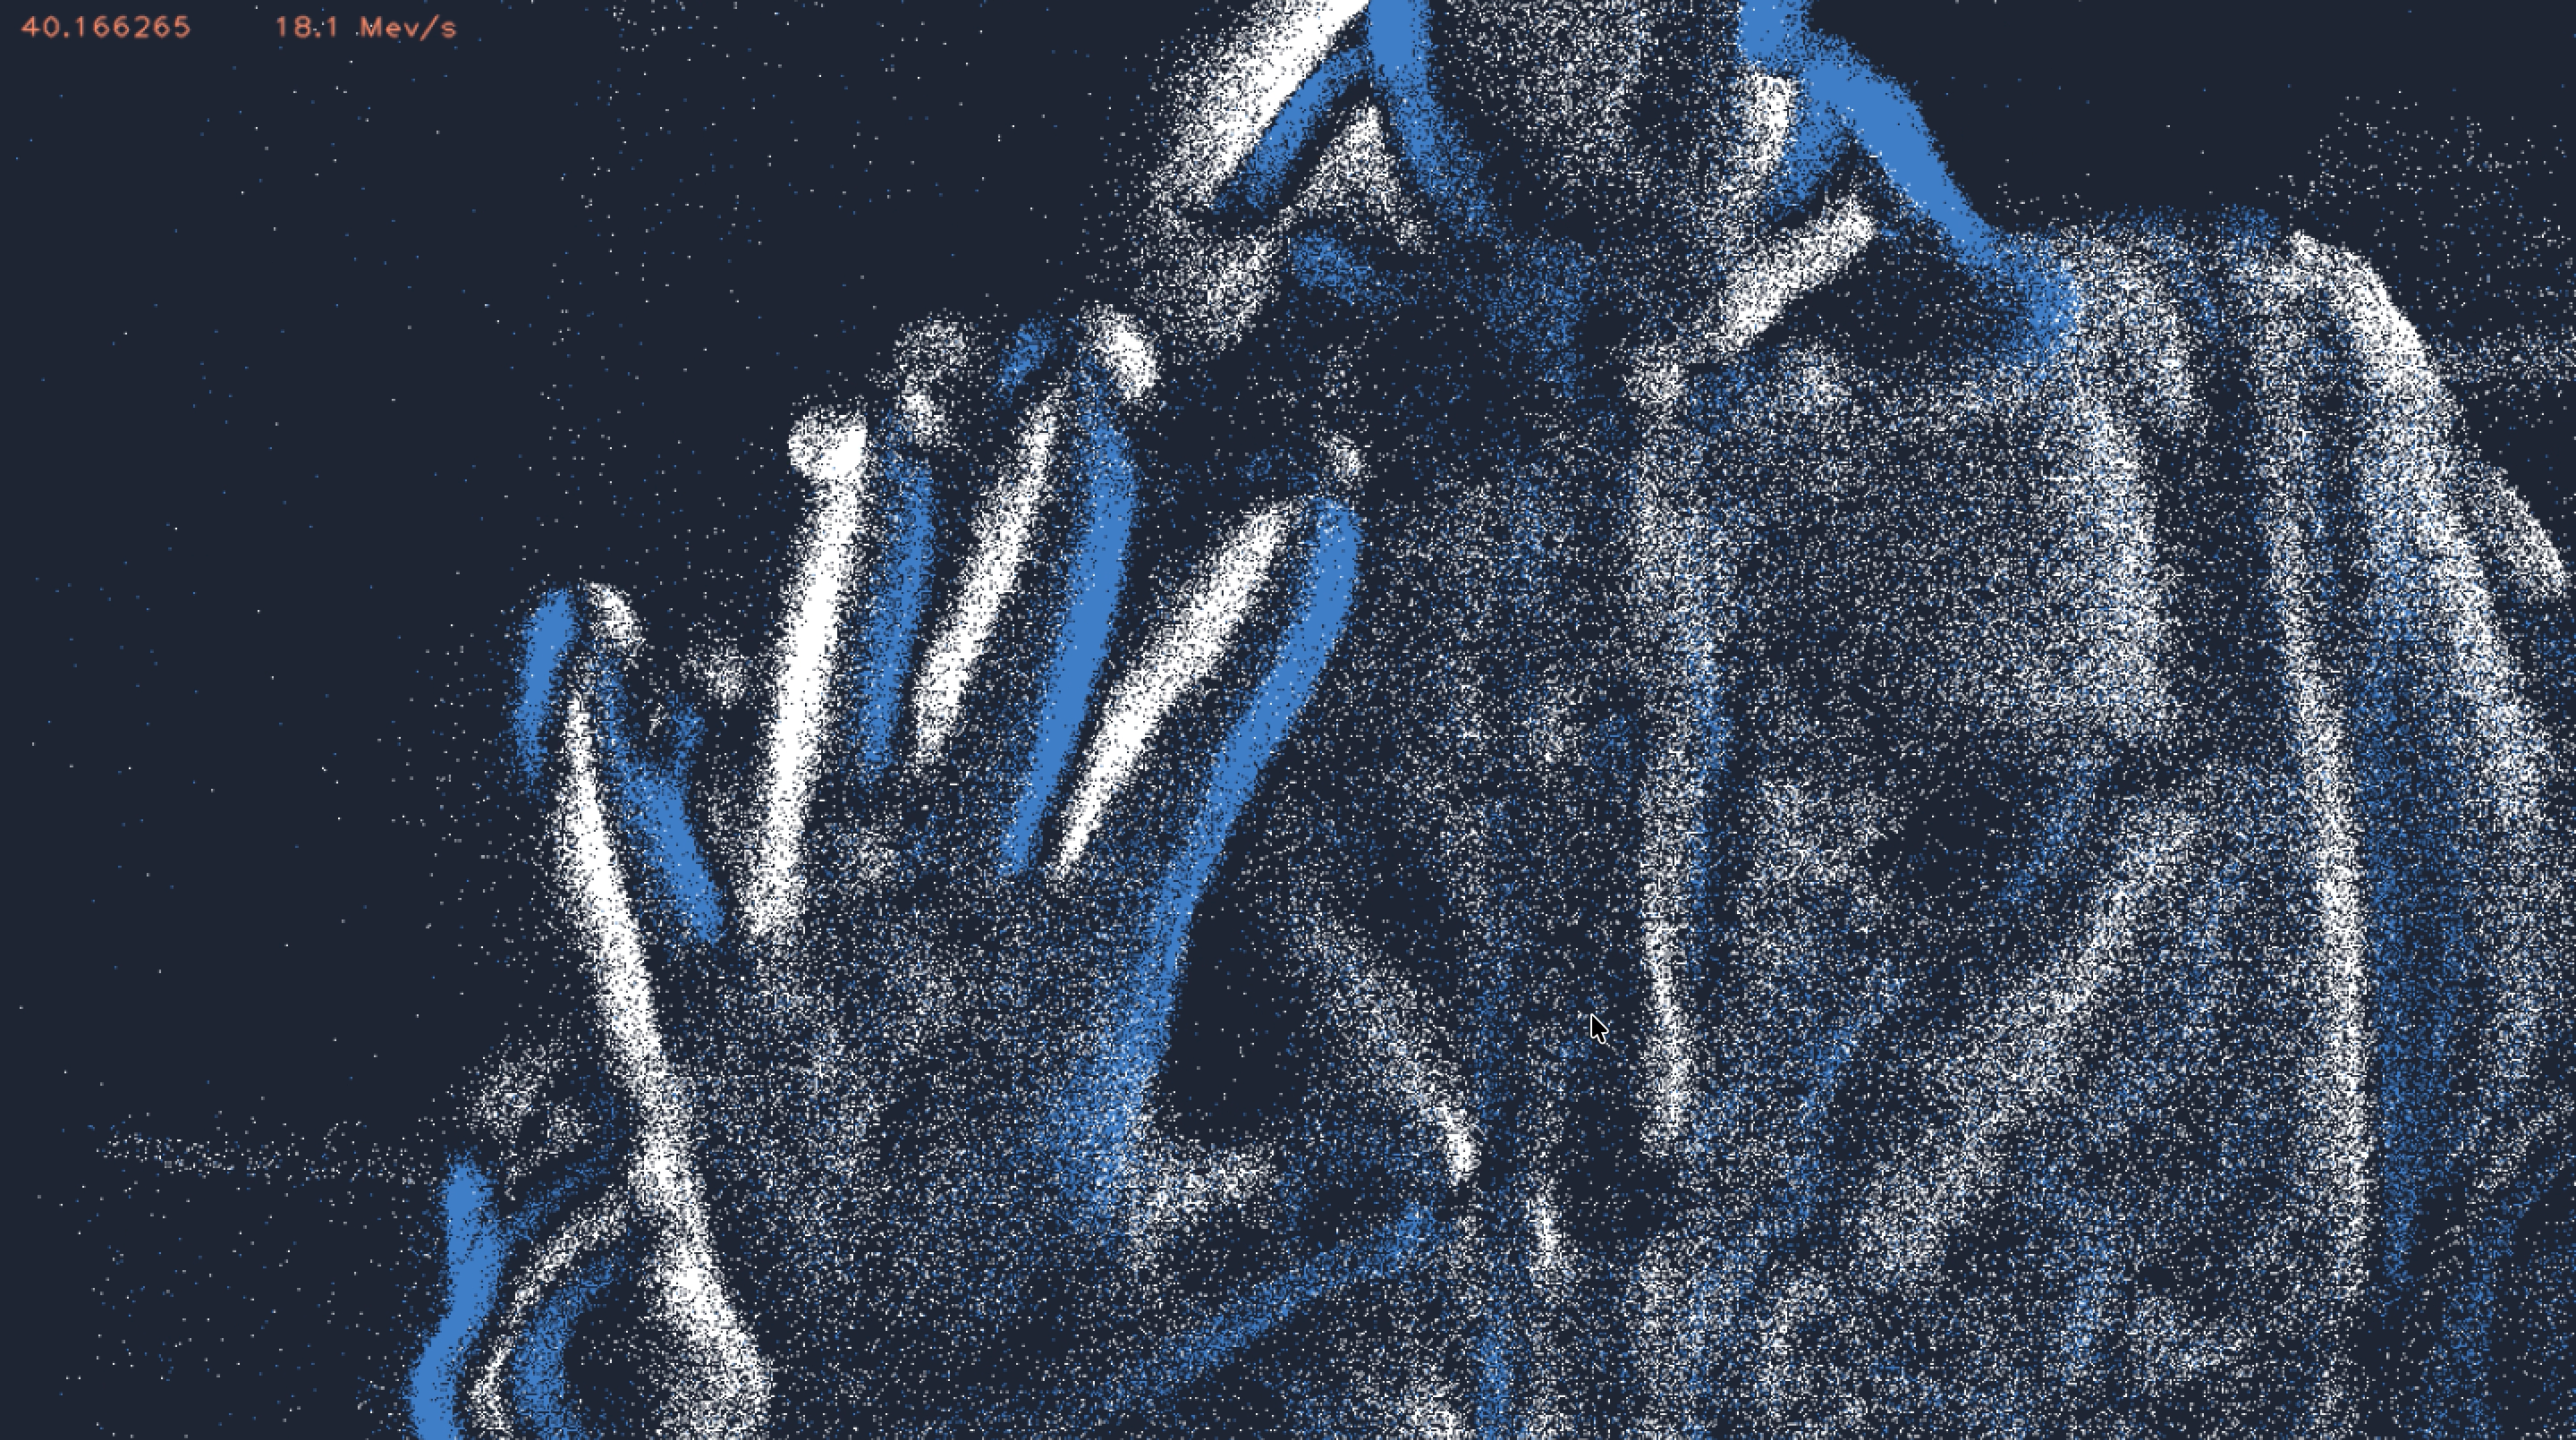
\includegraphics[width=\linewidth]{images/kria_local_event_hand.png}
        }{
            \fbox{\parbox[c][0.20\textheight][c]{0.92\linewidth}{\centering Image to be uploaded: \texttt{kria\_local\_event\_hand.png}}}
        }
        \caption{Moving-hand scene}
    \end{subfigure}
    \hfill
    \begin{subfigure}[t]{0.48\textwidth}
        \centering
        \IfFileExists{images/kria_local_event_scene.png}{
            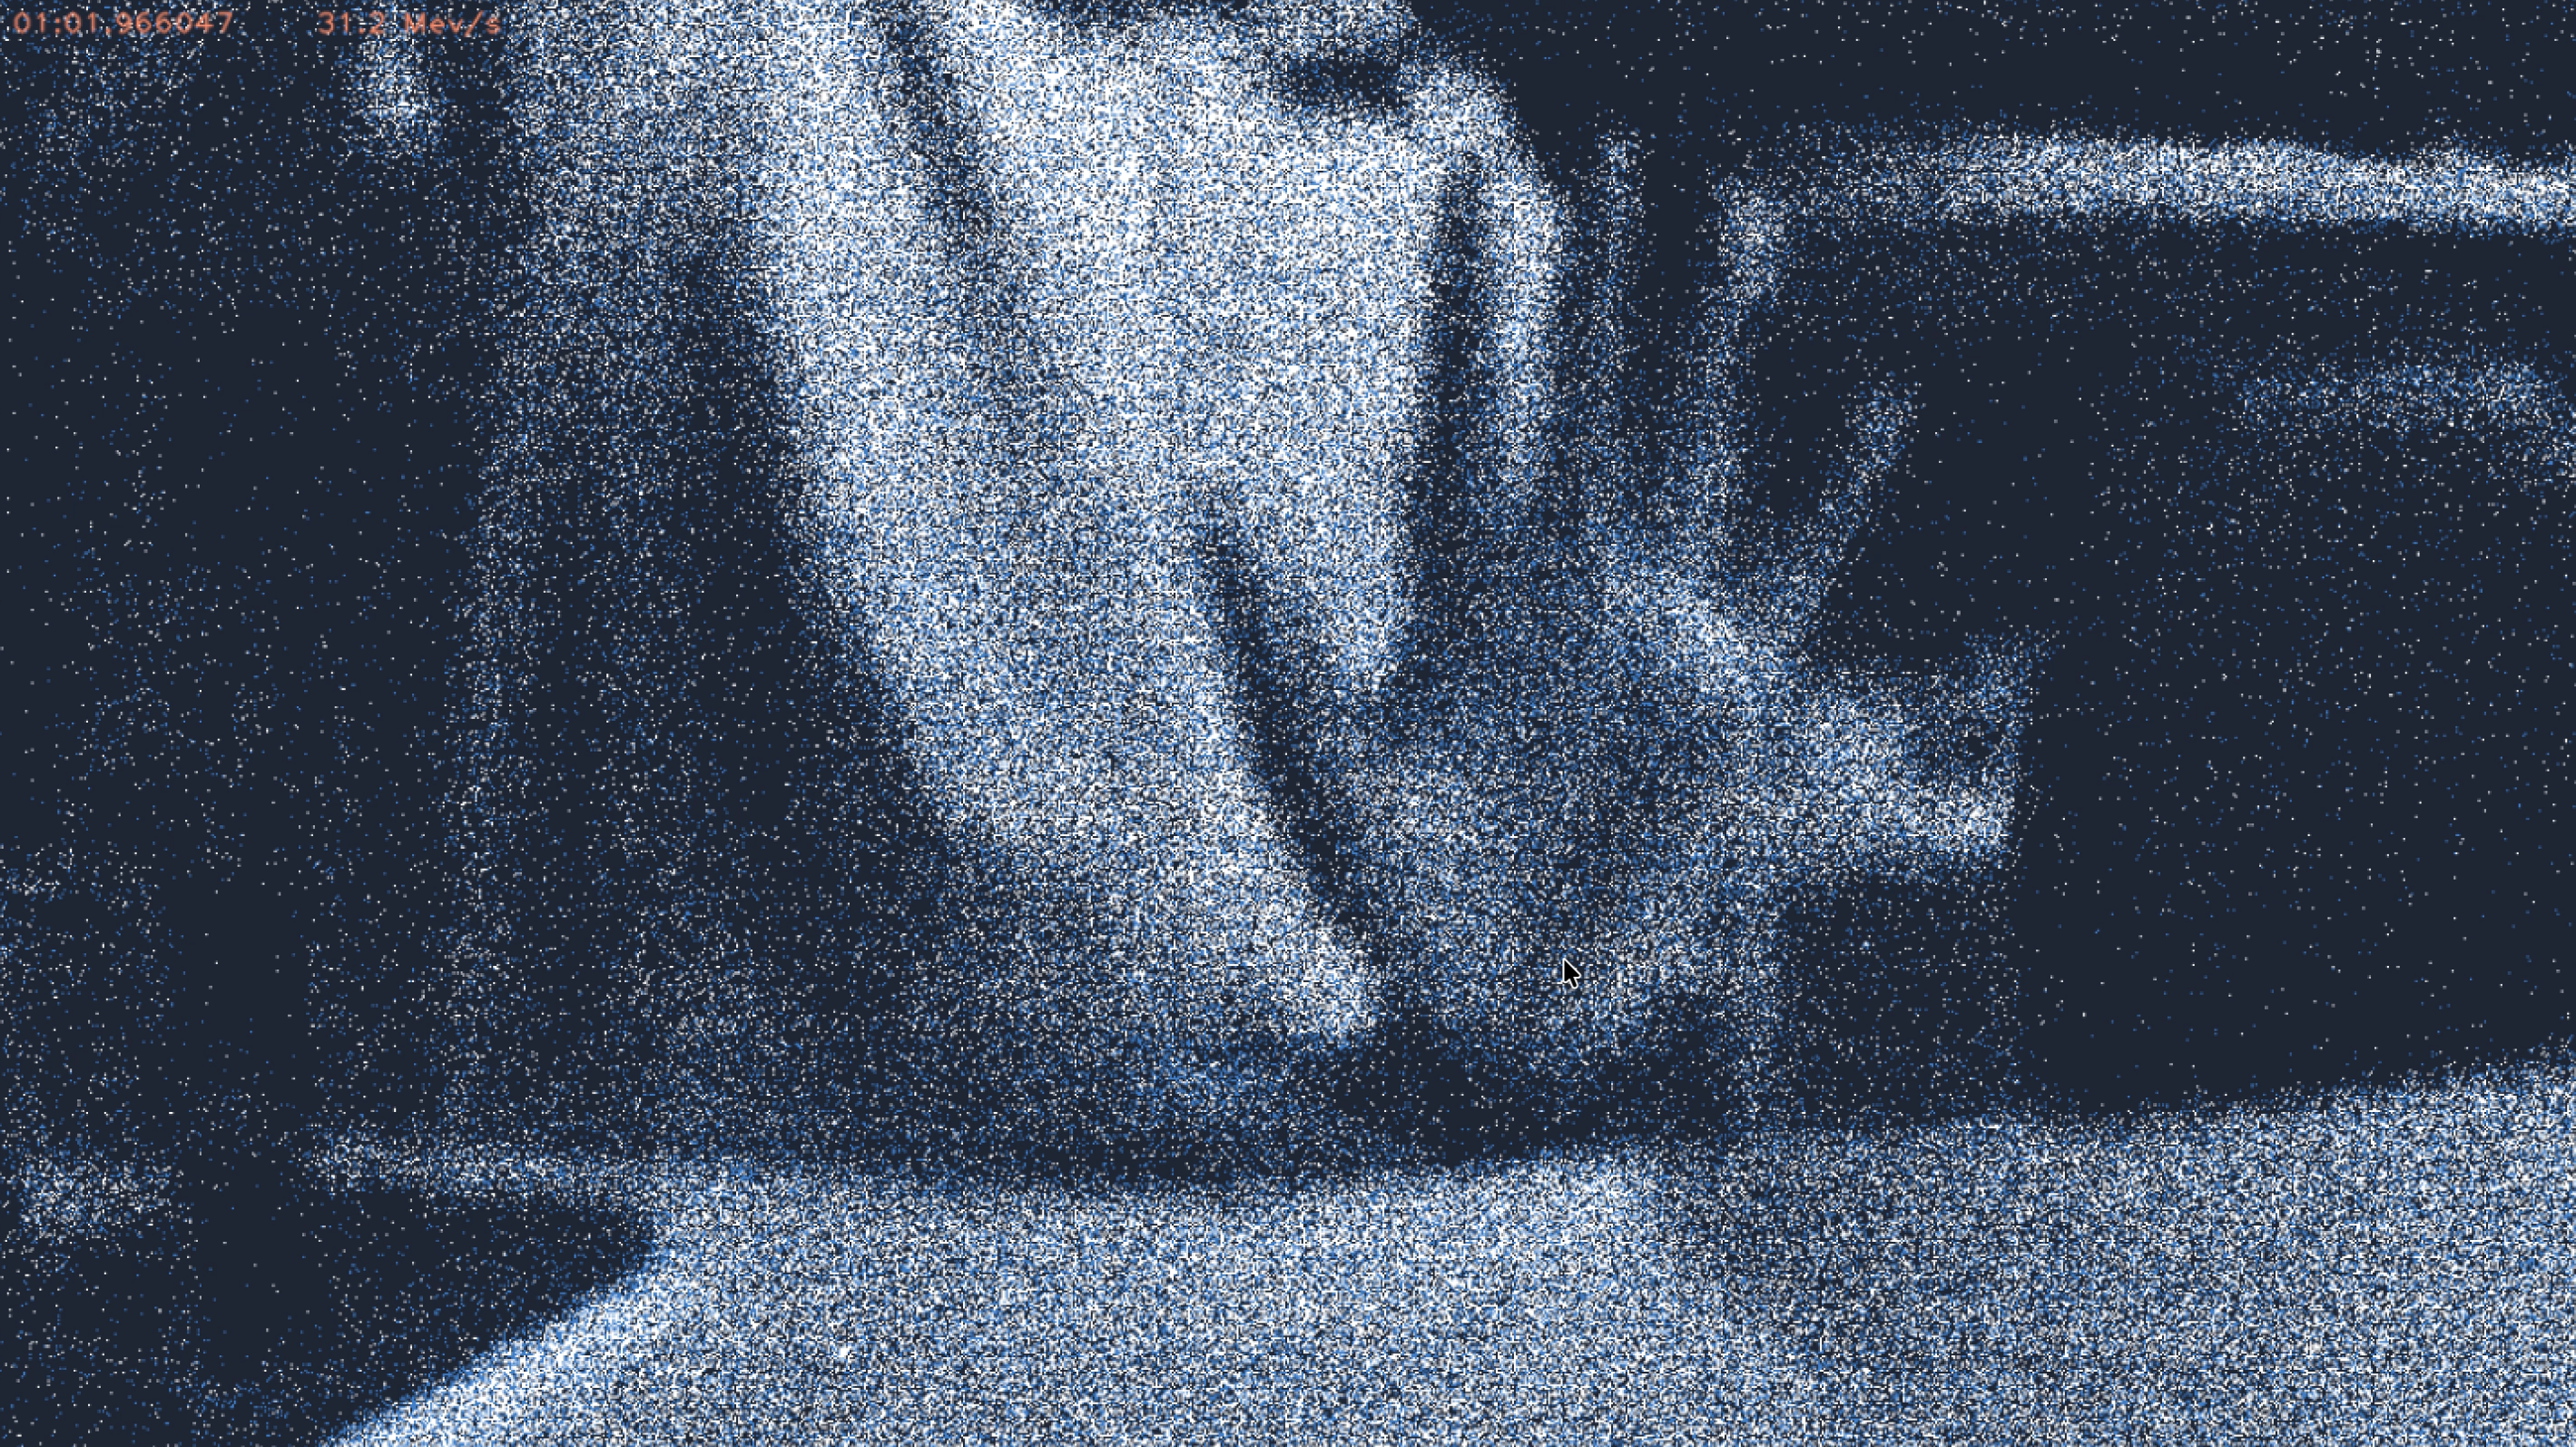
\includegraphics[width=\linewidth]{images/kria_local_event_scene.png}
        }{
            \fbox{\parbox[c][0.20\textheight][c]{0.92\linewidth}{\centering Image to be uploaded: \texttt{kria\_local\_event\_scene.png}}}
        }
        \caption{Indoor scene}
    \end{subfigure}
    \caption{Local visualization of the IMX636 event stream on the Kria KV260 using Metavision Viewer.}
    \label{fig:kria_local_event_stream}
\end{figure}

To further confirm the low-level data path from the camera to the Kria, the physical test used the \texttt{v4l2-ctl} control with \texttt{/dev/video0} at a resolution of 1280$\times$720. Then, 100 V4L2 buffers were captured directly from \texttt{/dev/video0}, producing a raw data file of about 17 MB. This shows that the data path from the IMX636 through the existing FPGA/V4L2 path can actually produce event data. To reduce the effect of V4L2 minor-number changes after reloading the FPGA overlay or rebooting the system, the current startup logic does not hard-code one fixed \texttt{/dev/v4l-subdevX}. Instead, it dynamically finds the corresponding subdevice from the IMX636 device name exposed by the kernel.

The final real-time test configuration in this work uses EVT3 as the event encoding published by the Metavision ROS 2 driver on the Kria. The driver also supports forwarding raw EVT21 event packets, but the final system in this report only uses EVT3. The driver combines the raw callback blocks returned by the camera into \texttt{EventPacket} messages. The current configuration publishes when either a 1 ms time threshold or a 262144-byte size threshold is reached. Therefore, the size of a single message is not fixed and changes with the event rate and raw-block boundaries. Sending raw event packets through the network instead of images rendered on the Kria allows the Jetson to keep access to the event data itself, while software decoding and image rendering are handled in one Docker runtime environment.

For the 1 GbE real-time link, the current default configuration also includes software traffic and event-rate control. The byte-rate limiter is set to 20,000,000 bytes/s with a 4 MiB burst, and the Metavision event-rate controller is set to 5,000,000 events/s. In the actual tests, without rate limiting, the Kria-to-Jetson network transfer showed clear stalling and data accumulation. Therefore, these parameters are mainly used to control the cross-device transfer load. Both the input queue and send queue use a limited length of 4 to reduce further data accumulation and memory growth. When the input queue is full, the system keeps the earlier unprocessed data and drops newly arriving raw blocks, while recording the dropped data in the statistics. Therefore, the continuous throughput of this system is measured under these software control parameters and does not represent the maximum unrestricted raw output capability of the sensor.

\section{Real-Time Event Processing System Between Kria and Jetson}

After the previous stages were completed, this project combined the real event camera, Kria front end, ROS 2 network communication, EVT3 decoding and rendering in Jetson Docker, and image display on the host into one continuous real-time processing pipeline. The final system uses a distributed structure. The Kria acquires event-camera data and publishes EVT3 \texttt{EventPacket} messages. Jetson Docker performs event decoding and image rendering. The Jetson host uses \texttt{rqt\_image\_view} to display the images produced by the renderer. This task division separates the sensor front end, network communication, event processing, and graphical display, so each module can be checked separately.

The overall experimental hardware setup is shown in Figure~\ref{fig:hardware_setup}. The data flow of the final system is shown in Figure~\ref{fig:final_realtime_pipeline}.

\begin{figure}[htbp]
    \centering
    \IfFileExists{images/hardware_setup.png}{
        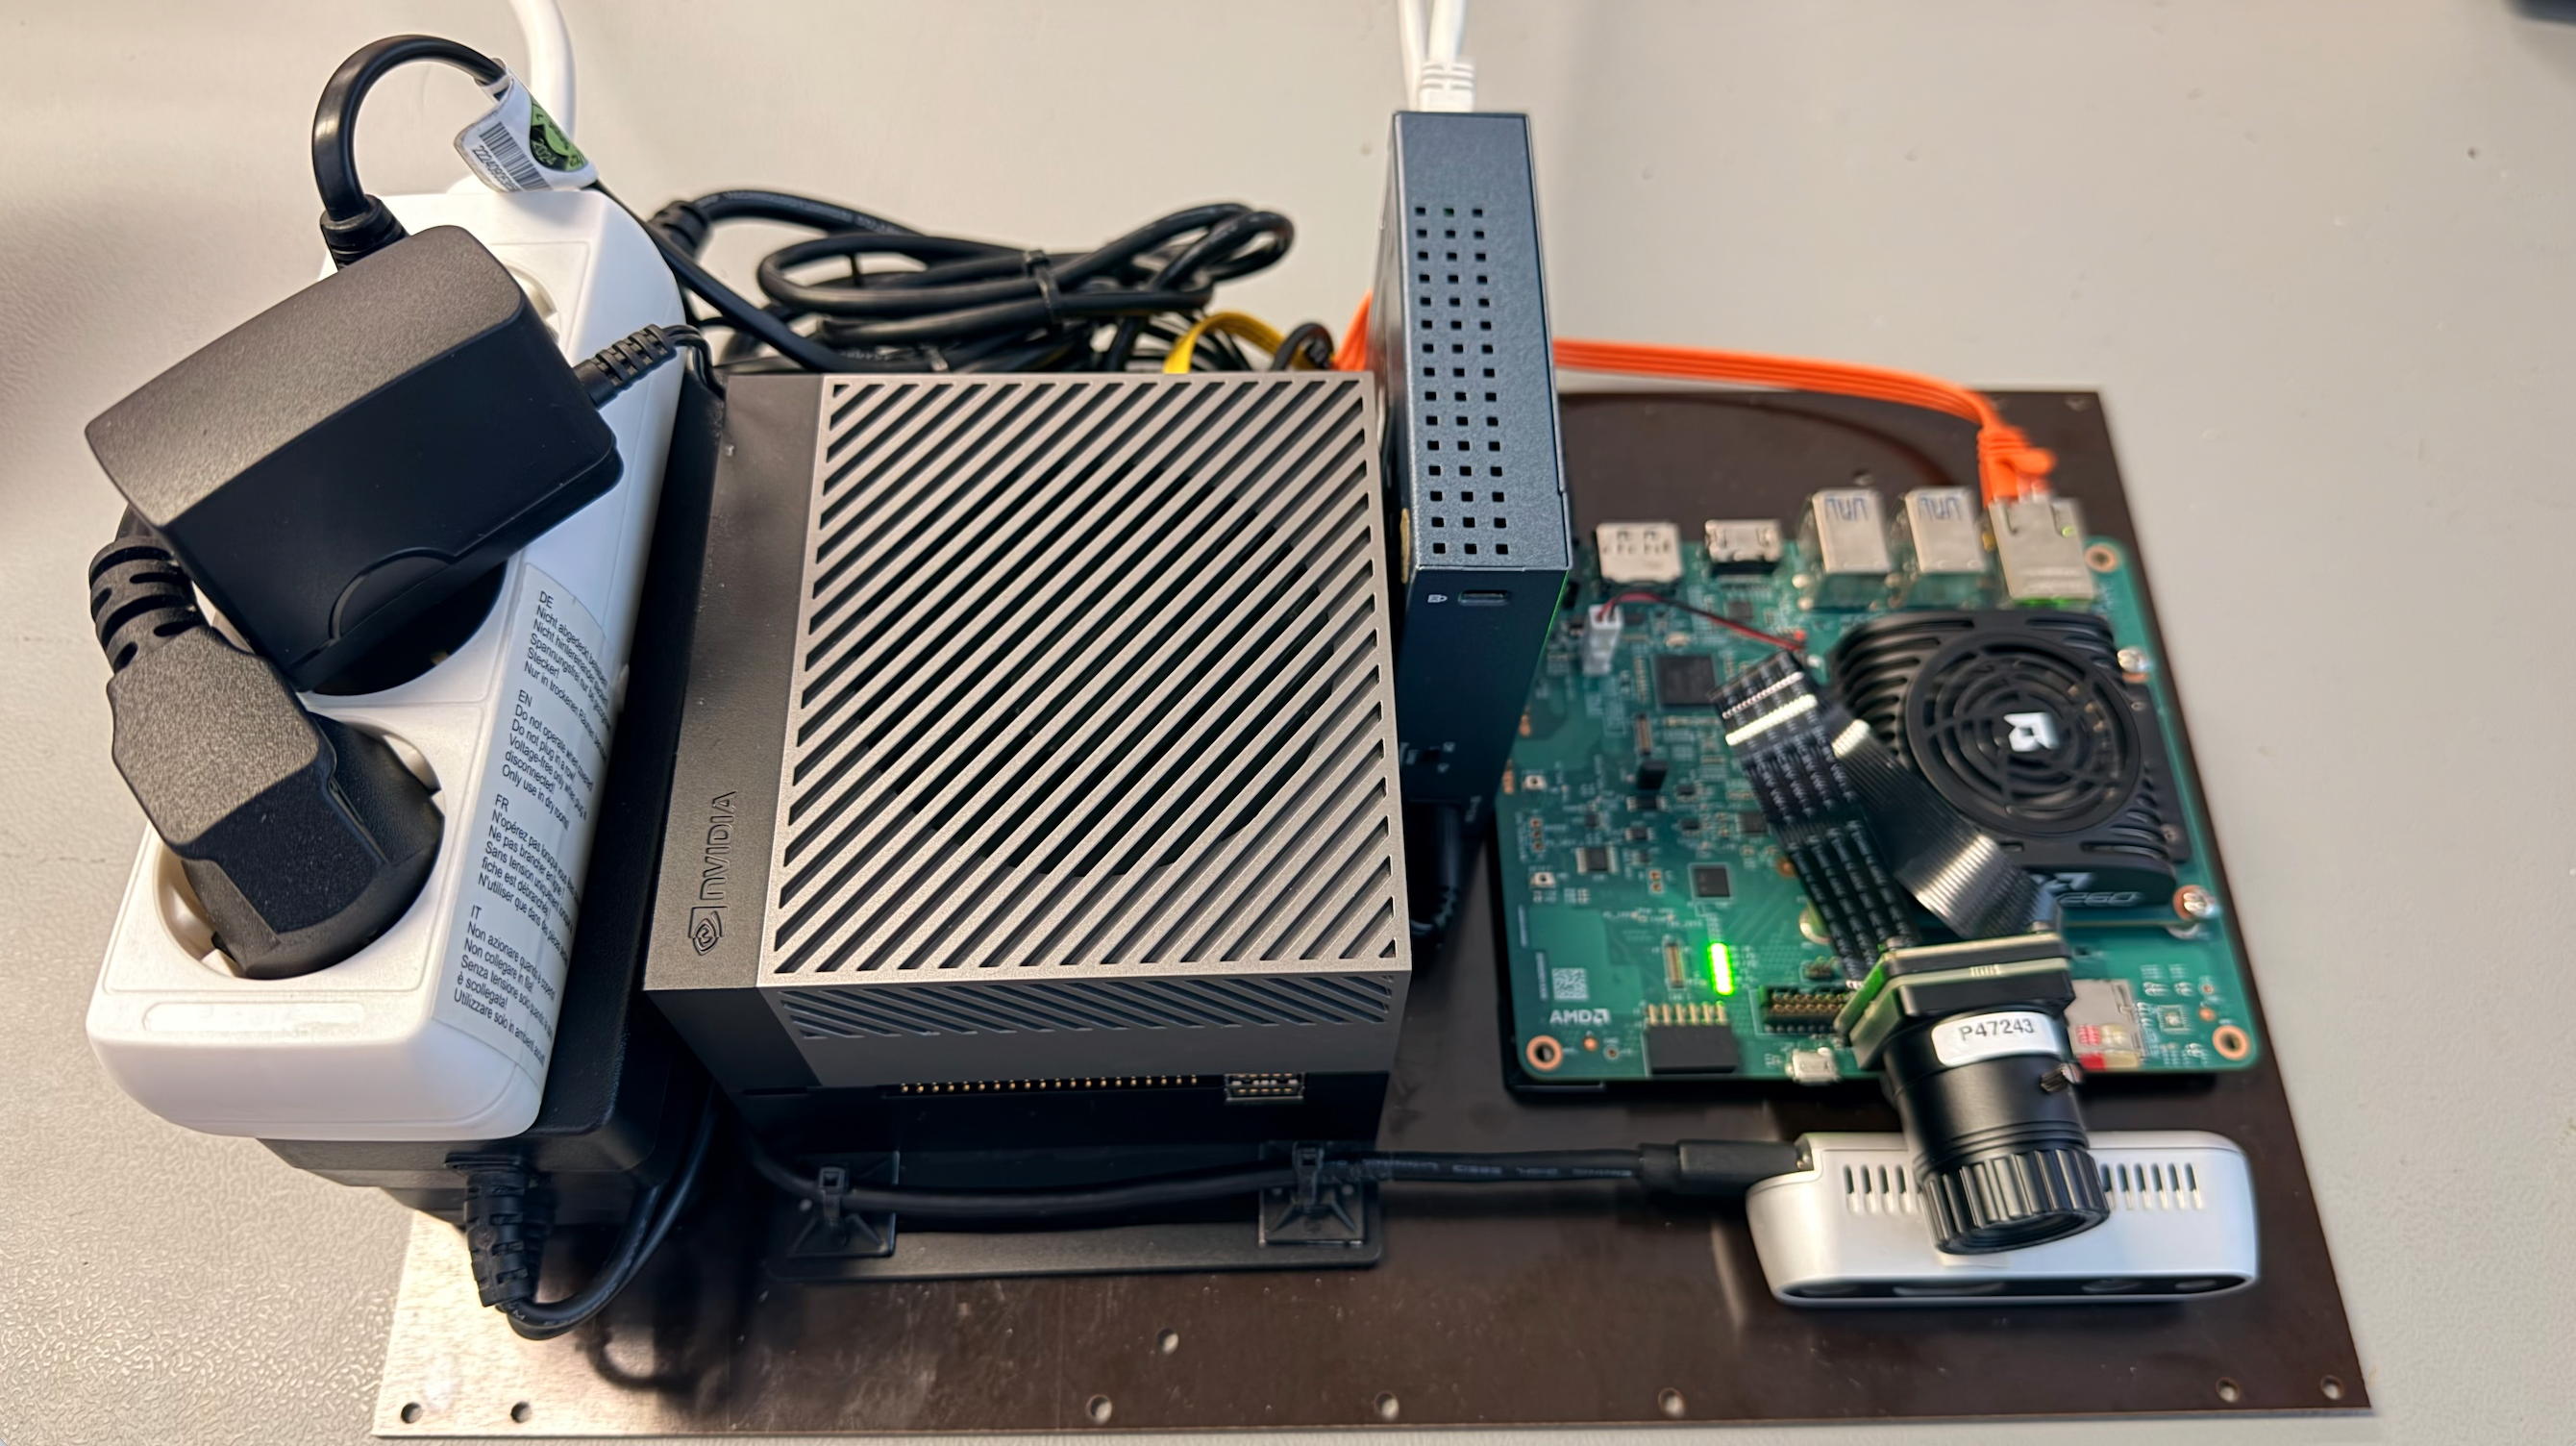
\includegraphics[width=0.86\textwidth]{images/hardware_setup.png}
    }{
        \fbox{\parbox[c][0.24\textheight][c]{0.82\textwidth}{\centering Image to be uploaded: \texttt{hardware\_setup.png}}}
    }
    \caption{Experimental hardware setup with Jetson Orin, Kria KV260, and the IMX636 event camera.}
    \label{fig:hardware_setup}
\end{figure}

\begin{figure}[htbp]
    \centering
\begin{tikzpicture}[
    >=Latex,
    box/.style={
        draw,
        rounded corners,
        align=center,
        minimum height=1.1cm,
        font=\small
    }
]

    % Top row
    \node[box, text width=2.0cm] (camera) at (-3,0)
        {IMX636\\
        Event Camera};

    \node[box, text width=2.8cm] (kria) at (1.8,0)
        {Kria KV260\\
        {\ttfamily Metavision}\\
        {\ttfamily ROS 2 Driver}\\
        {\ttfamily EVT3}\\
        {\ttfamily EventPacket}};

    \node[box, text width=2.1cm] (network) at (8.7,0)
        {Ethernet\\
        ROS 2};

    % Bottom row
    \node[box, text width=3.2cm] (docker) at (6.1,-3.4)
        {Jetson Orin\\
        Docker\\
        \texttt{event\_camera\_codecs}\\
        \texttt{event\_camera\_renderer}};

    \node[box, text width=2.5cm] (host) at (1,-3.4)
        {Jetson Host\\
        \texttt{rqt\_image\_view}};

    % IMX636 -> Kria
    \draw[->]
        (camera.east) --
        node[midway, above, font=\scriptsize]
        {MIPI-CSI}
        (kria.west);

    % Kria -> Ethernet / ROS 2
    \draw[->]
        (kria.east) --
        node[midway, above, yshift=-1mm, font=\scriptsize]
        {\texttt{/metavision\_driver/events}}
        (network.west);

    % Ethernet / ROS 2 -> Jetson Docker
    \draw[->]
        (network.south) |-
        (docker.east);

    % Jetson Docker -> Jetson Host
    \draw[->]
        (docker.west) --
        node[midway, above, font=\scriptsize]
        {image topic}
        (host.east);

\end{tikzpicture}
    \caption{Final real-time event processing pipeline from the IMX636 event camera to visualization on Jetson.}
    \label{fig:final_realtime_pipeline}
\end{figure}

ROS 2 provides cross-device modular communication in this system. The \texttt{metavision\_driver} on the Kria acts as a publisher and publishes the event topic. The event-processing components in Jetson Docker subscribe to this topic, and the messages are transferred between the two devices over Ethernet. The important point for the system is that the camera driver and Jetson processing modules are separated through a standard ROS 2 topic. This allows the publisher, network transfer, and subscriber/renderer status to be checked separately.

The Metavision ROS 2 driver on the Kria obtains events from the IMX636 data path and publishes them as \texttt{EventPacket} messages with the EVT3 encoding used in the current test~\parencite{metavisionDriver}. The final event topic is \path{/metavision_driver/events}, and the message type is \texttt{event\_camera\_msgs/msg/EventPacket}. The publisher uses \texttt{best\_effort}, \texttt{volatile}, and KeepLast QoS settings, which are more suitable for continuous high-throughput sensor data.

The Kria and Jetson exchange ROS 2 \texttt{EventPacket} messages over Ethernet. As long as both devices are in a network environment where they can communicate and use consistent ROS 2 settings, the subscriber in Jetson Docker can receive the EVT3 event packets published by the Kria. By keeping the network communication layer as a standard ROS 2 topic, the renderer, recording node, or future event-based object detection module on the Jetson can be replaced later without changing the camera driver on the Kria.

On the Jetson side, Docker is used to provide one ROS 2 event-processing runtime environment. Inside the container, \texttt{event\_camera\_codecs} processes the EVT3-encoded events inside the \texttt{EventPacket}, while \texttt{event\_camera\_renderer} directly subscribes to the event data and accumulates and renders the events into normal image messages~\parencite{eventCameraRenderer}. \texttt{event\_camera\_codecs} provides the event-encoding parsing function, while \texttt{event\_camera\_renderer} converts the decoded events into images that are easier to observe.

The image topic generated by the renderer is \path{/metavision_driver/renderer/image_raw}. It is subscribed to and displayed by \texttt{rqt\_image\_view} on the Jetson host. Keeping the renderer inside Docker and the graphical interface on the host separates the ROS 2 and event-camera software environment from the desktop display environment, while the image topic continues to be used as the interface between them. The final validation showed that \texttt{rqt\_image\_view} could continuously display images generated from the real IMX636 event stream.
